\documentclass{article}
\usepackage[T1]{fontenc}
\usepackage{lmodern}
\usepackage{graphicx}
\usepackage{amsmath,amssymb}
\usepackage[a4paper,margin=2cm]{geometry}
\usepackage[absolute,overlay]{textpos}
\setlength{\TPHorizModule}{1mm}
\setlength{\TPVertModule}{1mm}
\usepackage[indonesian]{babel}
\usepackage{hyperref}
\setlength{\emergencystretch}{2em}
% unit: Halaman 10

\begin{document}

% === Halaman 10 (llm) ===

% (tidak ada teks dari model)

% deskripsi: Diagram hierarki yang menunjukkan berbagai Mode Operasi (Modes of operation) enkripsi blok, termasuk Electronic codebook (ECB), Cipher block chaining (CBC), Cipher feedback (CFB), Output feedback (OFB), dan Counter (CTR).
% bbox normalisasi: [0.7700, 0.3450, 0.9200, 0.6650]
\begin{textblock*}{31.50mm}(161.70mm,102.46mm)
\noindent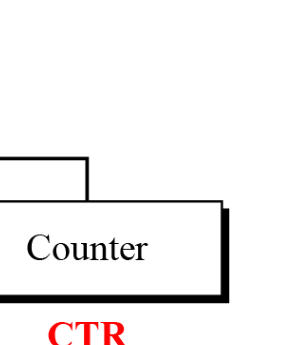
\includegraphics[width=31.50mm,height=95.04mm]{../../images/llm/page_010_img_01.png}%
\end{textblock*}

\end{document}
